\documentclass[11pt]{amsart}
%%% WARNING: Do NOT change the page size, fonts, or margins!  Penalties will apply.

\usepackage{graphicx, hyperref}
\usepackage{amssymb,amsmath,amsthm, mathtools}
\usepackage{placeins} %enables \FloatBarrier, that prevents floats from going below it.
\usepackage{caption}
\usepackage{subcaption}
\usepackage{algpseudocode, algorithm}
\usepackage{tikz}
\usepackage{physics}
\usepackage[T1]{fontenc}
\usepackage{DejaVuSansMono}
\usetikzlibrary{arrows}
\usetikzlibrary{tikzmark}
\usepackage{listings}
\usepackage{float}

% Define style for Python code snippets
\lstset{
    language=Python,
    basicstyle=\small\ttfamily, % Set font size to small
    frame=single, % Add frame around code snippets
    showstringspaces=false % Don't show spaces in strings
}

%%% WARNING: Do NOT change the page size, fonts, or margins!  Penalties will apply.
%%% WARNING: Do NOT change the page size, fonts, or margins!  Penalties will apply.

% Some macros for ease of use
\newcommand{\R}{{\mathbb R}}
\newcommand{\A}{{\mathrm{A}}}


\begin{document}
\title{Adapting Bayesian Filters for use with Circular Data}
\author{Cannon Tuttle, Curtis Evans, Spencer Ashton, Tyler Sanders}

%% comment out next command to put today's date after names of group members, or put a desired day in the parethesis
\date{\today}

\begin{abstract}
We adapt Bayesian filtering methods for use with circular data. We focus on a specific acoustics application, but accurate angle estimation is crucial in several fields. Due to the wrapping property of circular data, traditional filters are unsuitable for filtering circular data. We employ a simple continuous state-space model and successfully adapt the Kalman and Particle filters to account for the nature of circular data. We test these methods on both simulated and real data, finding our filters to perform far superior to an unmodified Kalman filter.
\vspace{-\baselineskip}
\end{abstract}
\vspace{-\baselineskip}
\maketitle
\vspace{-\baselineskip}
\section{Problem Statement and Motivation}
Imagine a construction site with heavy machinery, such as excavators, dump trucks, etc.,  in operation. The machine operator typically communicates with designated spotters via radio, but this leaves any other workers on the site unable to interface directly with the machine operators. A BYU acoustics project seeks to remedy this with a sound system that can pick up on the sound of human voice from outside the machine, filter out the noise, and reproduce the speech, including its relative direction to the machine, for the machine operator.  This will augment the safety of those outside the machinery by increasing the awareness of the machine operators.

In order to replicate the directionality of the sound, the angle of arrival of the sound must be accurately estimated over time. Currently, this angle in relation to the center of the microphone array (see Figure \ref{fig:array}) is calculated using pressure measurements and triangulation. Distance is also calculated, but is unimportant for this application. According to the researchers, a sufficiently good angle approximation for this application is within $\pm15^{\circ}$ of the true angle. However, the noisy environment makes raw triangulation insufficiently accurate. Somewhat rudimentary filtering has been implemented to improve stability, but so far the results of the calculation are still unreliable.

\begin{figure}[htp]
\includegraphics*[width=0.5\textwidth]{Pic of Real Mic Array.jpg}\hfill
\caption{Microphone array used in data collection.}
\label{fig:array}
\end{figure}

Our aim is to improve the robustness of the angle estimation in order to allow the researchers to more accurately reproduce the sound directionality. Previous work has shown that an unmodified Kalman Filter does not work well on circular data \cite{Research}. Various distributions, including a wrapped normal distribution and the Von Mises distribution have been successfully implemented to be used with Kalman type filters. However, these adaptations are complex and not easily implemented, as they include approximating the distributions with a wrapped Dirac mixture \cite{Research}. Particle filters have shown to be useful for filtering angle data, for example in robotics \cite{Oops}.

We modeled the angle of arrival evolution process as a continuous state space model and employed various Bayesian filtering techniques in order to optimize the angle estimation. This included adapting Kalman filters, normally used with data defined for all real numbers and gaussian distributed noise, to work with circular data that are defined on $[0,2\pi]$ with the wrapping property at the boundary. We also adapted a Particle filter, a type of Bayesian filter that allows for the use of an arbitrary distribution, for use with circular probability distributions.

%% Second Section
\section{Data}
The data used for this project included both data given to us by the research team and simulated data. The original data is in the form of microphone pressure measurements that we then ran through a triangulation algorithm, provided to us by the research team, to produce angle measurements in time. Due to symmetry, each pair of microphones produces two possible angles. These can each be taken directly as possible measurements, producing 42 measurements per time step in our case, or all synthesized in order to produce a single angle measurement per time step. The provided triangulation algorithm produces data for both cases.
However, the provided data didn’t include certain extreme scenarios relevant to this application, including harsh discontinuities, frequent angle wraparounds, etc. To account for these scenarios, we produced representative synthetic data by plotting a “true” angle, then adding gaussian noise to it to be used as the angle measurement. We also reserved real data to test our filter on after tuning our filter parameters.

%% Third Section 
\section{Methods}
We utilized several methods to compute the hidden angle measurement. Throughout this paper we use degrees in plots and examples, but all the measurements and computations were done in radians. 

\subsection{State Space Model}
In order to represent the angle evolution over time, we used a state space model that included current angle, previous angle, and angular velocity. In this case, the speaker will either be stationary or moving near a constant velocity, so we did not include an acceleration term. Angular velocity was approximated as $\theta'_t \approx \frac{\theta_{t} - \theta_{t-1}}{\Delta t}$ and $\theta_t$ was approximated using the forward Euler step $\theta_t \approx \Delta t\theta’_{t}$. This yields the following:

\[\mathbf{x}_t = \begin{pmatrix*}[l]
    \theta_t \\
    \theta_{t-1} \\
    \theta'
\end{pmatrix*},\;  
F = \begin{pmatrix*}[l]
    1 & 0 & \Delta t \\
    1 & 0 & 0 \\
    \frac{1}{\Delta t} & \frac{1}{\Delta t} & 0
\end{pmatrix*},\;
H = \begin{pmatrix*}[l]
    1 & 0 & 0 \\
    \vdots & \vdots & \vdots\\
    1 & 0 & 0

\end{pmatrix*}\]
 where $H$ is dimension $n\times3$ for $n$ observed angles. The state evolution is
 \[\mathbf{x}_t = F\mathbf{x}_{t-1} + \mathbf{w}_t,\]
\[\mathbf{z}_t = H\mathbf{x}_t + \mathbf{v}_t.\]
All of our filters used the same state evolution equations.

\subsection{Kalman Filter}
We implemented two Kalman Filter \cite{V3}\cite{V3 Lab Manual} approaches. We term the Kalman filter illustrated in the textbooks the naïve Kalman filter and the our altered version the circular Kalman filter.

\subsubsection{Naïve Kalman Filter}
We first implemented a naïve Kalman filter using the efficient Kalman Gain form. In the update step, the state estimation is updated as follows, where $K_t$ is Kalman Gain: \[\mathbf{\hat{x}}_t = \mathbf{\hat{x}}_{t|t-1} + K_t(\mathbf{z}_t - H\mathbf{\hat{x}}_{t|t-1}).\] The quantity $\mathbf{z}_t - H\mathbf{\hat{x}}_{t|t-1}$ is the difference between the observation, $\mathbf{z}_t$, and expected observation given the predicted state, $H\mathbf{\hat{x}}_{t|t-1}$. The naïve Kalman filter computes this as an arithmetic difference, however, it would be more accurate to compute a circular difference, as no two angles are more than $180^{\circ}$ apart. This is illustraded by the examples in the table below:

% TODO fix the spacing on the first row of the table
\begin{center}
    \begin{tabular}{||c c c c||}
     \hline
     Observed & Expected Observation & Arithmetic Diff & Circular Diff \\ 
     \hline\hline
     $15^{\circ}$ & $355^{\circ}$ & $-340^{\circ}$ & $20^{\circ}$ \\ 
     \hline
     $355^{\circ}$ & $15^{\circ}$ &  $340^{\circ}$ & $-20^{\circ}$ \\
     \hline
     $120^{\circ}$ & $90^{\circ}$ & $30^{\circ}$ & $30^{\circ}$ \\ [1ex] 
     \hline
    \end{tabular}
    \end{center}



\subsubsection{Circular Kalman Filter}
We adapted the Kalman filter for circualr data by changing the aforementioned update step to account for circular arithmetic. Specifically, we changed the calculation of the difference between true and expected observations to ensure that the difference calculated was never greater than $180^{\circ}$ (i.e. measuring the distance between angles on a circle), while preserving sign to account for their relative position. This computes the circular difference illustrated in the table. The new update step is illustrated in Algorithm \ref{alg:kalman}.


\begin{algorithm}
    \caption{Altered Update Step}\label{alg:kalman}    
    \begin{algorithmic}
        \State $\mathbf{v} \gets \mathbf{z}_t - H\mathbf{x}_t$
        \If{$\lvert{\mathbf{v}}\rvert \geq \pi \;\textbf{and}\; \mathbf{v}\leq 0$} 
            \State $\mathbf{v} \gets \mathbf{v} + 2\pi$
        \ElsIf{$\lvert{\mathbf{v}}\rvert \geq \pi \;\textbf{and}\; \mathbf{v} \geq 0$} 
            \State $\mathbf{v} \gets \mathbf{v} - 2\pi$
        \EndIf 
        \State $\tilde{\mathbf{y}_t} = \mathbf{v}$ 
        \end{algorithmic}
    \end{algorithm}

%% Insert some pictures of the angle adjustment and add the algorithm 

\subsection{Particle Filter}
The second method we employed was another type of Bayesian filter, the particle filter \cite{Particle}. The particle filter employs a large number of possible current states, each referred to 
as a “particle”. Each particle has an associated weight, interpreted as the probability that the particle accurately reflects the hidden state. All weights sum to 1 to form a probability distribution. As the source can possibly 
come in at any angle, we initialize the particles with uniformly distributed states and weights. At each time step, the filter propagates all of the particles forward in time according to the state space 
model, including adding state noise in the update step. Then, using the data, it updates the weights of each particle by computing the posterior probabilities given data. Finally, it computes the state estimate 
as the weighted average of the states of all the particles. 

In the update step, the filter computes $P(\theta|\text{data}) \propto P(\text{data}|\theta)P(\theta)$ for each particle. The prior $P(\theta)$ is given by the particle’s previous weight, while $P(\text{data}|\theta)$ is calculated 
according to the probability distribution defined for the measurement noise. One of the benefits of the particle filter is that, unlike the normal distribution requirement of the Kalman filter, any arbitrary noise 
distribution may be employed. In this case, we used the Von Mises distribution (see Figure \ref{fig:particle_filter_stuff}, right side). This closely approximates a Normal distribution 
that is “wrapped” around the angle boundary between $0$ and $2\pi$. Thus, no other consideration of angle wrapping must be made for the particle filter. After the posterior weights have been calculated, they are again normalized by 
their sum so they represent a probability distribution.

\begin{figure}[htp]
    \centering
    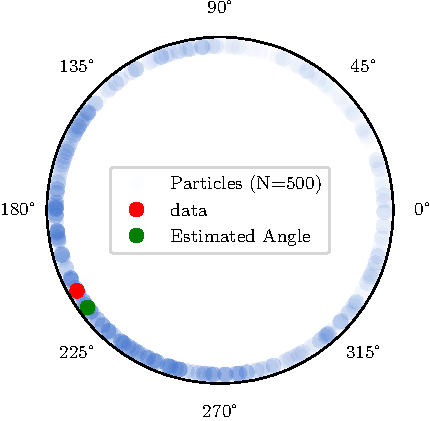
\includegraphics[width=0.45\textwidth]{actual_paper_graphs/particle_filter_example.pdf}\hfill
    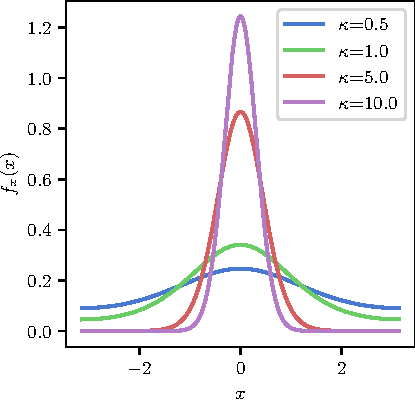
\includegraphics[width=0.45\textwidth]{actual_paper_graphs/von_mises_pdf.pdf}\hfill
    \caption{Left, an example particle filter at a given timestep. The particles are colored according to weight, with the heaviest weights clustering around the data angle. Right, the Von Mises distribution for various shape parameters ($\kappa$).}
    \label{fig:particle_filter_stuff}
\end{figure}

Particle filters suffer from what is called the "Degeneracy Problem", in which the weights become concentrated in a small number of the total particles. This is solved by resampling, a process in which low probability particles are replaced 
with higher probability particles. Detailing this problem and its solution is beyond our scope, but we used the \lstinline{systematic_resample} function from \lstinline{filterpy} to accomplish resampling.

As the particle filter keeps track of a large number of possible states around the circle, it is much more flexible to nonlinear behavior. This is desirable in our case, as a source may possibly reappear at any 
location in the state space. Unfortunately, the particle filter performs a similar number of computations for each individual particle as the Kalman filter performs in total. As we are using \lstinline{n_particles}, our particle filter takes \lstinline{n_particles} 
times as long to compute each step.

The Particle filter is defined with the following hyperparameters: \lstinline{K1} defines the shape term of the state noise distribution,  \lstinline{K2} defines the same for the measurement noise distribution, \lstinline{n_particles} defines the number of particles the model employs, and \lstinline{n_eff_particles} defines the minimum number of “effective” particles allowed before particles are resampled. We tuned the hyperparameters by performing a
gridsearch over several different possible values using the metrics discussed below. A filter was constructed for each hyperparameter
combination, with its performance tested across multiple datasets. We then chose the
model that produced minimum average circular error over the different datasets (see Figure \ref{fig:particle_hyperparam}).

\begin{figure}[htp]
    \centering
    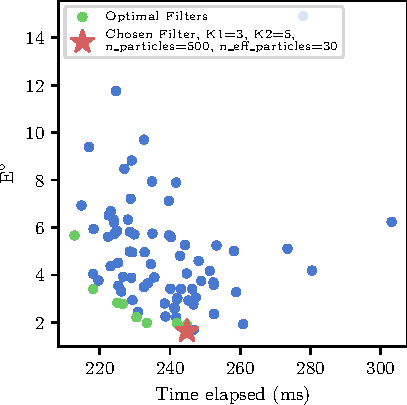
\includegraphics[width=0.45\textwidth]{actual_paper_graphs/gridsearch_particle_filter.pdf}\hfill
    \caption{Hyperparameter tuning of the Particle filter. Any filters colored green may be considered "optimal".}
    \label{fig:particle_hyperparam}

\end{figure}

\subsection{Evaluation Metrics}
We also used the average absolute angle error as our primary evaluation metric. This took the average of the absolute circular difference between the true state and predicted state at each time step across the whole dataset. We referred to this as average circular error, \lstinline{E}. We also used the total time to filter a given dataset as our other evaluation metric. We refer to this as filter time, \lstinline{T}.

\section{Results and Analysis}
We examine the success of the circular Kalman Filter (Figure \ref{fig:simple_kalman}), 
review filtering several simultaneous angle observations(Figure \ref{fig:multiple_angles})
, then consider the speed and accuracy of the various filters (Figures \ref{fig:all_simulated} and \ref{fig:all_real}).
Note, the figures best illustrate the results and performance of each filter.

\subsection{Circular vs Naïve}
As a simple demonstration, we compared the performance of the naïve and circular Kalman filters in tracking a source moving continuously in a circle. The circular Kalman filter modification resulted in a marked improvement in behavior across the boundary between $360^{\circ}$ and $0^{\circ}$ as 
compared to the naïve filter. The naïve filter tended toward the arithmetic mean of $180^{\circ}$ of the data, while the circular Kalman filter accurately tracked the source around the entire circle. See Figure \ref{fig:simple_kalman} below.


\begin{figure}[htp]
    \centering
    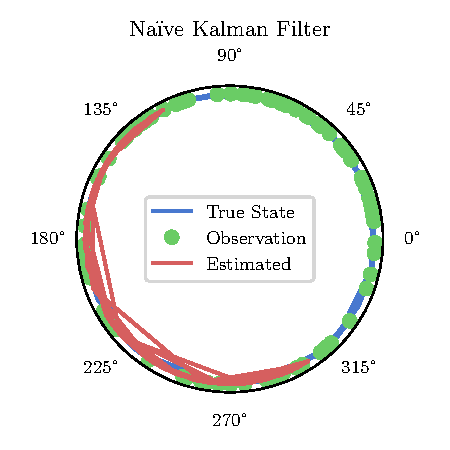
\includegraphics[width=0.45\textwidth]{actual_paper_graphs/non_altered_kalman.pdf}\hfill
    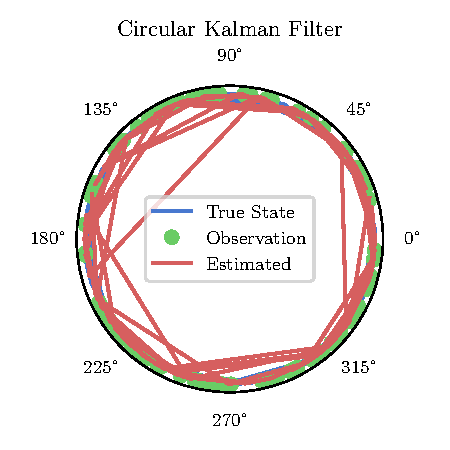
\includegraphics[width=0.45\textwidth]{actual_paper_graphs/altered_kalman.pdf}\hfill
    \caption{Naïve vs Circular Kalman Filter performance}
    \label{fig:simple_kalman}
\end{figure}

\subsection{Filtering Multiple Angle Estimates}

As discussed in Data, each microphone pair technically calculates two possible measured angles, which are normally synthesized by the provided triangulation algorithm to find the most likely angle. Since the observation matrix $H$ allows for an arbitrary number of measurements, we attempted filtering using all 42 angle measurements directly in our filters.  
See Figure \ref{fig:multiple_angles}. 
With this data, the Kalman filters failed to accurately track the data in any of the measured datasets. We believe this is because the array is not symmetric with respect to the angle of arrival of the sound, leading to angle measurements that are not distributed normally around the true angle. However, if the microphone array were to be circular, this method may be viable. In all other cases we treated the one angle returned by the triangulation algorithm as the measurement angle. The Particle filter successfully tracked the real angle in this case, and even ignored certain abberations that were returned by the single measurement operation. However, incorporating this number of measurements caused the specified particle filter to take ~$\frac{1}{3}$ as long as the total length of the data, possibly reaching filter times unsuitable for real time filtering.

\begin{figure}[htp]
    \centering
    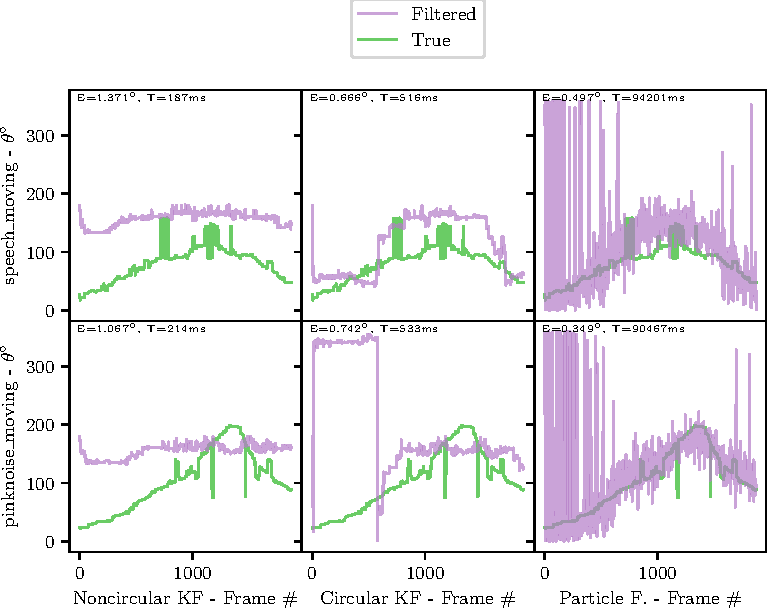
\includegraphics[width=.75\textwidth]{actual_paper_graphs/multiple_angles.pdf}\hfill
    \caption{Filtering various real data with multiple simultaneous angle measurements. The triangulation estimate angle (green) is output from the provided triangulation algorithm. The estimated angle (pink) is being filtered.}
    \label{fig:multiple_angles}
\end{figure}

\subsection{Speed}
The Kalman filters ran in about 3-5ms on 1 second of data, while the Particle filter took about 125ms, in total about $30$ times longer than the Kalman filters.
Thus, all of our filters can run in real time. 

\subsection{Accuracy}
We tested the accuracy of the filters on the following synthetic and real datasets. See Figures \ref{fig:all_simulated} and \ref{fig:all_real} for quantitative results, as well as the discussion below. Note that on the real datasets, the true angle is unknown.
\begin{figure}[htp]
    \centering
    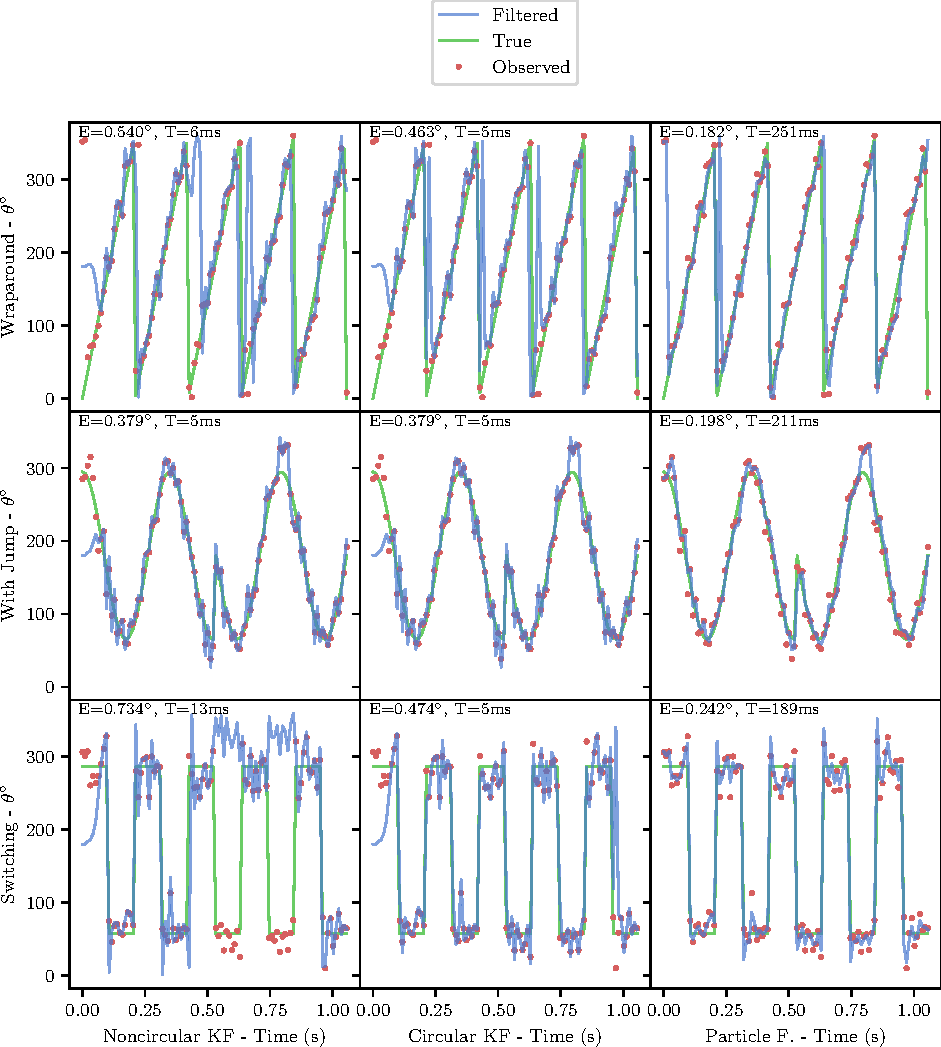
\includegraphics[width=.95\textwidth]{actual_paper_graphs/all_simulated.pdf}\hfill
    \caption{
        Running each filter (columns) on various simulated datasets (rows).
        The red dots represent observations of the green true angle. 
        The observations alone are filtered to produce the blue estimate angles.
        Each cell displays average error (E) and the total time taken, in seconds (T).
        }
    \label{fig:all_simulated}
\end{figure}

\subsubsection{Wraparound}
This is a synthetic dataset that represents a source moving in a circle at a constant angular velocity to test a simple case involving wraparound. This was also the data used in \ref{fig:simple_kalman}. As discussed above, the Naïve Kalman filter failed to track the angle, while the Circular Kalman filter successfully navigated the wraparound point. The particle filter also accurately tracked the angle around the wraparound.
\subsubsection{With Jump}
This is a synthetic dataset that represents a source moving back and forth then switching trajectory midway in order to account for a simple nonlinearity. Since there was no wraparound to consider, the Naïve and Circular Kalman filters both had equivalent performance, both accurately tracking the angle. The Particle filter tracked the angle about twice as accurately as the Kalman filters.
\subsubsection{Switching}
This is a synthetic dataset that represents the nonlinearity of jumping between angles across $0^{\circ}$. The Naïve Kalman filter performed poorly on this dataset. The Circular Kalman and Particle filters performed much better, with the Particle filter being about twice as accurate as the Circular Kalman filter.
\begin{figure}[htp]
    \centering
    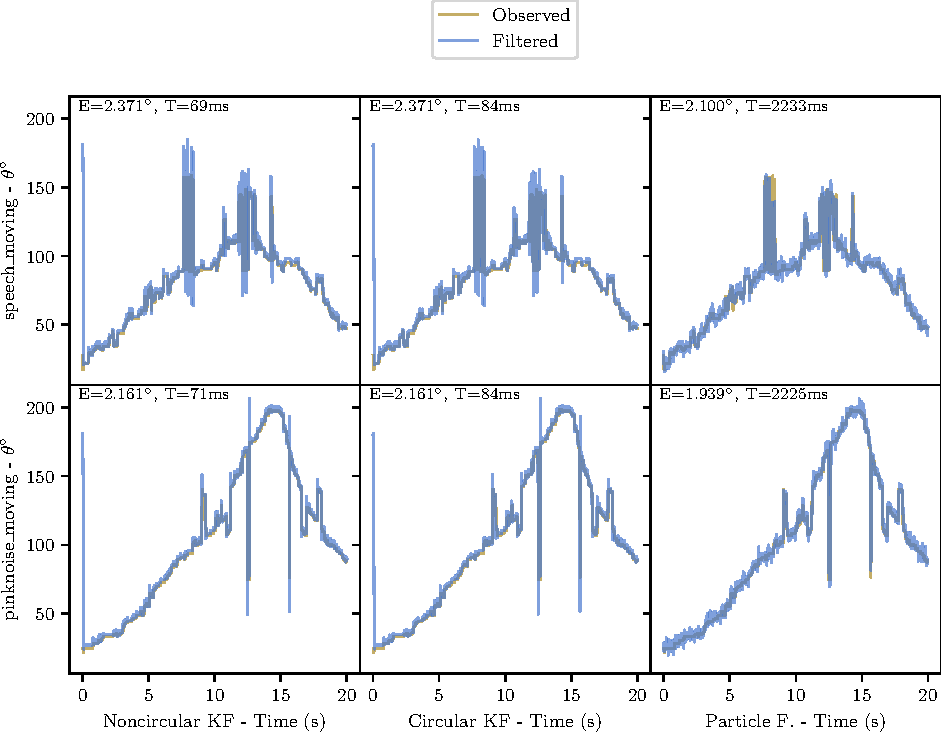
\includegraphics[width=.75\textwidth]{actual_paper_graphs/all_real.pdf}\hfill
    \caption{Running each filter (columns) on various real datasets (rows). Observed angles (yellow) are calculated using triangulation. The observed angle is then filtered (blue).}
    \label{fig:all_real}
\end{figure}
\subsubsection{Pink Noise Moving}
This dataset is a recording of a source producing pink noise, a type of filtered gaussian noise, while moving around the microphone array. All three filters behaved well on this dataset, with the particle filter again being slightly more accurate. 
\subsubsection{Speech Moving}
This dataset is a recording of a source producing pink noise, a type of filtered gaussian noise, while moving around the microphone array. All three filters accurately tracked the source in this dataset, with the particle filter performing slightly more accurately.

\section{Ethical Considerations}
Although there are no data privacy concerns, we must consider the safety of operators using direction-filtered cabin audio in heavy machinery. Before deployment, this model must be 
shown to be a net positive to safety, despite operator risk compensation (acting less carefully because of perceived safety features \cite{Risk}). Even then,
operators should still use sight and radio communication to identify nearby individuals, and people near machinery must still exercise caution. 

\section{Conclusion}
Our goal was to improve robustness of the angle estimation by adapting filtering methods for use with circular data. We derived a very simple modification to the Kalman filter that 
allows it to work for circular data, and we implemented a particle filter using circular probability distributions. We found the particle filter and the circular Kalman filter suitable 
for circular data. The particle filter handles nonlinearities well but comes at a computational cost, while the circular Kalman filter is computationally efficient but has its 
accuracy suffer in cases of strong nonlinearity. The Particle filter was around twice as accurate across all datasets as the Circular Kalman filter, but took about 30 times longer to run. If enough computing headroom is available, the Particle filter is a suitable choice for this application, but the Circular Kalman filter also performed well with very few computations. Only the Particle filter was consistently within the desired $15^{\circ}$ of accuracy on all datasets. Due to the wraparound property of circular data, the naïve Kalman filter is unsuitable for circular data.

For the BYU Acoustics project specifically, if the computational cost of the filtering step is a concern, we would recommend use of the circular Kalman filter for this project due to its low 
cost and accurate performance except in cases of strong nonlinearity. If more computational headroom is allowed, the particle filter would be ideal, as it performed well even in cases of 
nonlinearities. Furthermore, the utility of these methods extends to any field in which angle measurements are taken, including robotics, navigation, and astronomy. The hyperparameters of our 
methods can easily be modified to adjust accuracy, flexibility, and computational cost depending on what is needed for the given scenario. 




%%%%%%%%%%%%%%%%%%%%%%%%%%%%%%%%%%%%%
%% Bibliography below
%%%%%%%%%%%%%%%%%%%%%%%%%%%%%%%%%%%%%
\FloatBarrier % Keep the figures from being put after the bibliography
\newpage
%% If using bibtex, leave this uncommented
%\bibliography{refs} %if using bibtex, call your bibtex file refs.bib
\bibliographystyle{alpha}

%% If not using bibtex, comment out the previous two lines and uncomment those below
\begin{thebibliography}{99}
\bibitem{Research} G. Kurz, I. Gilitschenski and U. D. Hanebeck, "Recursive nonlinear filtering for circular data based on circular distributions," \textit{2013 American Control Conference}, Washington, DC, USA, 2013, pp. 5439-5445, doi: 10.1109/ACC.2013.6580688.
\bibitem{V3} The ACME Volume 3 Textbook
\bibitem{V3 Lab Manual} J. Humpherys and T. Jarvis, "Labs for Foundations of Applied Mathematics, Volume 3, Modeling with Uncertainty and Data."
\bibitem{Particle} Labbe, Roger. “Kalman and Bayesian Filters in Python”.
\bibitem{Risk} Masson, Maxime; Lamoureux, Julie; de Guise, Elaine (October 2019). "Self-reported risk-taking and sensation-seeking behavior predict helmet wear amongst Canadian ski and snowboard instructors". \textit{Canadian Journal of Behavioural Science.} 52 (2): 121–130. doi:10.1037/cbs0000153. S2CID 210359660.
\bibitem{Oops} I. Marković and I. Petrović, "Speaker localization and tracking with a microphone array on a mobile robot using von Mises distribution and particle filtering," \textit{Robotics and Autonomous Systems}, Volume 58, Issue 11, 2010, pp. 1185-1196, doi: 10.1016/j.robot.2010.08.001
\end{thebibliography}

\end{document}